\chapter{自然语言理解:从语言到逻辑}{From Language to Logic}
\label{chap:comprehension}

本章阐述如何对第\ref{chap:intro}章中的提到的假设1展开研究。根据该假设,我们认为, 借助于依存关系语法和传统逻辑与谓词逻辑的合理结合,将自然语言表达式转换成满足下列两个条件的逻辑表达方式是完全可行的:
\begin{itemize}
\item 包含该自然语言表达式的主要语义
\item 具体化自然语言表达式中存在的任何无法在语言到逻辑的转换消除的歧义,使得这些歧义能通过基于语境知识的逻辑推理后很直截了当地得到消除。
\end{itemize}

基于这样的假设,我们采用的自然语言方法是,首先利用链语法分析工具Link Parser\cite{Sleator1993},然后在此基础上搭建了一个用于依存关系抽取的工具RelEx,最后开发了一个新的逻辑关系抽取工具RelEx2Logic,通过超图的同态映射方式将句法结构转换成语义表示。该方法概念上的本质并不依赖这些特定的工具,而是具体的实现方法。

确切地说,如何将“自然语言理解系统”分解成不同模块以及如何进行不同模块之间的转换,取决于对语言学理论的选择。在2008-2012年期间,OpenCog中的自然语言理解模块采用如下流程:

\begin{verbatim}
文本 --> 分词/断句 --> 基于链语法的句法分析(Link Parser) --> 依存关系抽取(RelEx)--> 基于FrameNet的语义关系抽取(RelEx2Frame) --> 语义节点和关系链(SemanticNodes & Links)
\end{verbatim}

2012年的时候我们对系统进行了一些简化,取消了对FrameNet的依赖,采用了如下的目前正在使用的系统:

\begin{verbatim}
文本 --> 分词/断句 --> 基于链语法的句法分析(Link Parser) --> 依存关系抽取(RelEx)--> 抽象的逻辑关系抽取(RelEx2Logic --> 语义节点和关系链(SemanticNodes & Links)
\end{verbatim}

需要注意的是,目前的很多自然语言理解系统都有“词性标注”阶段,在我们目前使用的方法中,词性标注被绑定在句法分析阶段,对于Link Parser来说,词性已被作为单词的一个属性定义在词典里。尽管如此,如果能在Link Parser里使用先进词性标注技术,无疑能减少不少字典编写方面的工作,也能在一定程度上指导句法分析过程,因此也是有一定存在意义的。

本文的工作已经表明,上述系统中的各模块操作都是可行的,只需针对每一步制定相应的规则,或者通过有监督的机器学习方法来学习相应的规则,来指导其中的操作。针对本文自然语言理解方面的以下几个额外事项将在未来的研究中被实现:
\begin{itemize}
\item 使得各个子流程中所使用的规则,能很自然地支持基于持续经验增长的修正和泛化。
\item 使得语义理解能根据特定的语境来指导规则的选择。
\item 知道何时该打破规则,而根据语义的直觉指导相关操作。
\end{itemize}

另外需要注意的一点是,当使用基于规则的方法时,在规则的设计需要特别注意规则的可扩展性和可普及性,因为随着系统的经验增长,原先设计的规则可能无法被满足。

本章接下来的章节会系统介绍我们使用的自然语言理解系统中的各个子系统的工作原理和方法。

\section{链语法}{Link Grammar}\label{sec:linkGrammar}

本小节主要介绍链语法的基本原理和方法,并分析了和语言形式主义的不同,同时指出其中的问题以及我们对其进行的一些改进。

链语法(Link Grammar)在1991年由 Daniel Sleator和Davy Temperley共同提出 \cite{Sleator1993}。它和被广泛应用的依存语法类似,但两者也有很大的不同,比如链语法中两个单词的连接是无序的,而依存语法中有依存和被依存关系。链语法允许句子中的链接有环状结构,而依存语法是不允许环的存在的。链语法更倾向于语法理伦的词汇主义。

链语法的核心是链语法词典(Link Dictionary),词典中的每一个词都记录着一些特点的链接要求,这些链接要求通过一系列具有特定逻辑排序的链接子(connector)组合成的公式(Formula)收录在词典的相应词条里,链接子包含名称和后缀(“+”或“-”),后缀表示该链接子的指向方向,“+”表示该链接子指向右,“-”表示该链接子。如果两个词需要合法连接,则要求两个词首先有相同名称的链接子,且左边单词的链接子的连接方向必须指向右,右边单词的链接子的连接方向必须指向左。

链语法分析器(Link Parser)是基于链语法的句法分析器。使用链语法分析句子的时候,句法分析器对句子中的每个单词去查询链语法词典得到每个单词的链接要求,根据这些链接要求进行相应的链运算,便得到句子的链语法结构。 链语法判断句子是否合法,除了需要满足句子所有单词的链要求外,还要满足以下四个原则:

\begin{itemize}
\item 平面性(Planarity),链之间不能互相交叉。
\item 连通性(Connectivity),句子中的每个单词都必须有链和其他至少一个单词相连,形成连通图。
\item 顺序性(Ordering),公式中较左边的链接子必须和距离单词较近的单词链接,反之,公式中较右边的链接子必须和距离单词较远的单词链接。
\item 排它性(Exclusion),一对单词之间同时不能有两条链链接。
\end{itemize}

下面我们借用Sleator和Temperley的“Parsing with a Link Grammar”\cite{Sleator1993}中使用的例句来解释链语法分析的操作过程。

\begin{center}
\textbf{The cat chased a snake.}
\end{center}

链语法分析器对上面的例子分析后产生如下结果:

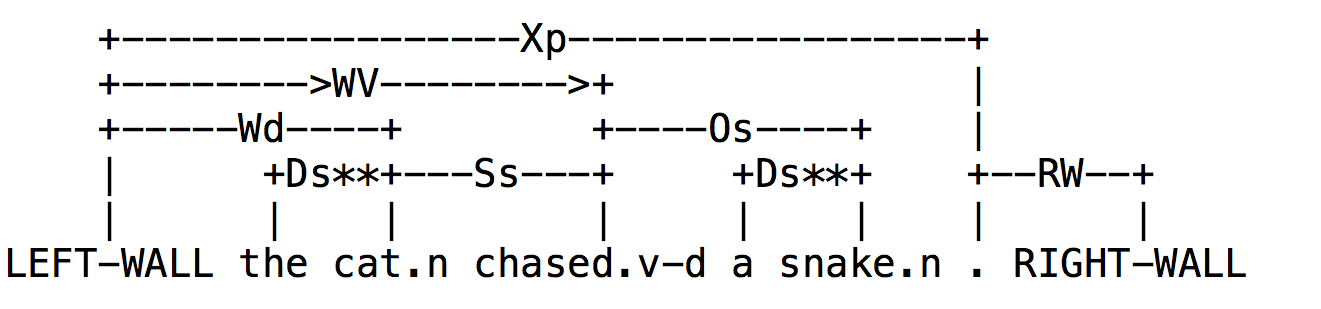
\includegraphics[width=12cm]{figures/catSnake.png}

由于我们对该链语法分析器做了不少的改进,所有我们这里给出的分析结果和Sleator和Temperley的原文中的结果以及发布在网上的分析器得到的结果会有细微的不同,后面章节会介绍我们做的改进。

链语法认为在句子最前面加上一个虚拟词(通常用LEFT-WALL表示)是很有必要的,这样首先能保证链语法的“连通性“原则,使得句子最后的标点符号能与LEFT-WALL连接而不被孤立。另外,在本文的\ref{sec:head}节也提到,通过这样的虚拟词来追溯句子的头(主动词)也是非常方便可行的。上面的句法分析结果中出现的”RIGHT-WALL”是可选的,可以用于特殊标点符号的处理,但通常情况下只是用RW链与句子最后的标点符号相连。

前面提到链语法词典是链语法的核心,它包含所有常用的英文单词的链接要求。下方的表格列出上述例句中出现的单词以及它们在链语法词典里被定义的链接要求。

\begin{tabular}{|p{2.0in}|p{2.1in}|} \hline 
\textbf{单词} & \textbf{公式} \\ \hline 
a, the & D+ \\ \hline 
snake, cat & D- \& (O- or S+) \\ \hline 
Chased & S- \& O+ \\ \hline 
\end{tabular}

如前面所述,链接要求限制了这些连接子必须按照一定的原则来分配,例如“the”只有一个向右的连接子D+,那么它只能和带有D-的单词形成合法的链接。而“snake”和“cat”都能和它相连,但根据链语法的“顺序性原则”,“cat”比“snake”近,所以“the”“cat”之间可以画一条D链,同样的道理,“chased”和“snake”之间可以画一条O链,以此类推。最终我们可以得到如下的结构图。需要注意的是,我们这里只是对链语法的工作原理做简单地介绍,因此忽略了链接子类型的子类型等细节,比如“cat”含有Ss+,“chased”含有链接子Ss-,,所以该句法结构图和我们上面列出的目前链语法分析器在连接类型上有点小出入。 

链语法分析器在对句子进行句法分析时,对句子中的每个单词,都会考虑下面两种变量:

\begin{itemize}
\item 该单词在链语法词典中对应的链接要求,即上面中的公式(Formula)
\item 该单词为了满足句子结构的一致性(Agreement)必须具备的特征属性
\end{itemize}

比如在上述例句中,对于单词“snake”,通过查询链语法词典,我们得到相应的公式“D- \& (O- or S+)”,同时该单词还有相应的特征属性如“时态(tense)”“人称(person)”等。但对于单词“the”,就不需要与一致性相关的变量。

链语法分析器中也使用简单的转换生成类似短语结构语法的句法分析结果,如下:

{\tt\begin{small}\begin{lstlisting}
(S (NP The cat)
	(VP chased
	 	(NP a snake))
 	.)
\end{lstlisting}\end{small}}

在我们的工作中,对该短语结构用的不多,所以这里不做详细说明。我们会在下一节简单讨论链语法和短语结构语法的潜在关系。

\subsection{链语法与短语结构语法}{Link Grammar vs. Phrase Structure Grammar}

讨论各种语法的优缺点不是本文的重点,本节只将链语法和典型的短语结构语法做个简单的对比来讨论它们的潜在联系。一般来说,依存语法和短语句法也有相应的联系(参见图\ref{fig:Dependency-and-Phrase-Structure}),但不同的依存语法使用不同依存关系集合,也有不同的属性,分析起来会比较复杂,也不是本文的研究内容,所以我们这里不做详细阐述。

\begin{figure}

\begin{centering}
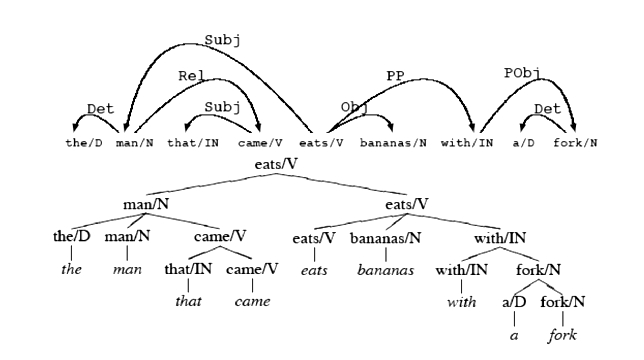
\includegraphics[width=12cm]{figures/schneiderFigure1} 
\par\end{centering}

\caption{依存句法分析和短语句法分析对比\label{fig:Dependency-and-Phrase-Structure}}
A comparison of dependency (above) and phrase-structure (below) parses.
In general, one can be converted to the other (algorithmically); dependency
grammars tend to be easier understand.
(图片来自G. Schneider, ``Learning to Disambiguate Syntactic
Relations''  Linguistik online 17, 5/03)\\
 \rule[0.5ex]{1\columnwidth}{1pt} 
\end{figure}

简单起见,这里只列出两条有用的观察结果,基于这些观察结果,我们不难发现,在链语法中也隐形存在短语结构。这是有一定道理的,但由于自然语言的复杂性,某些情况下可能也不是那么简单。

\begin{itemize}
\item 链语法中的公式是符合语法范畴的。例如,前面提到的例句中“chased”的链结构是“S- \& O+”,在范畴语法中,这意味着,“chased”属于这样的语法范畴,该范畴中的词都满足链结构“S- \& O+”。换句话说,链语法中每一个“公式”都对应依附该公式的单词的范畴。 
\item 词之间的链接也可以看成是短语的核心词(head)之间的链接。例如,在例句“The cat chased a snake”中,“chased”和“snake”之间有链接O,那么也可以说,以“chased”为核心词的短语和以“snake”为核心词的短语之间有链接O。换句话说,可以理解成,链语法为了简化,通过核心词来识别短语。
\end{itemize}

\subsection{识别句子的中心词}{Identifying the Head of a Sentence}
\label{sec:head}

链语法从词的局部着手关注任意两个词之间的关系,在一定程度上忽略了语言的层次结构。因此标准的链语法也存一些弊端,有不少语言现象会被链语法拒绝认为是不合法的结构。比如并列结构、介词短语等。在本文的研究过程,我们对链语法做了很多的改进,由于链语法的链接要求非常复杂,修改链语法词典可能牵扯到很多语言学上的问题。但这不是本文的研究重点,所以这里不一一列出我们做过的改进,只简单的列出几项较大的改进:

\begin{itemize}
\item 改进了链语法对连词的处理
\item 改进了链语法对量词的处理
\item 识别句子的中心词。
\end{itemize}

链语法分析器(Link Parser)是一个开源工具,包括链语法词典,我们所有的改进都发布在 \url{http://abisource.com/projects/link-grammar/}

为了读者对如何修改链语法词典有个大致的思路,本小节就其中的改进“识别句子的中心词”展开讨论。

对于“识别句子的中心词”的改进,我们的出发点是使链语法分析结构(Link Parse)能转换成一颗类似的依存句法树。改进后,我们能直接通过追溯“WV”链找到句子的中心词,或者通过追溯“CV”链找到子句的中心词。找到中心词后,可以将其定为树的根节点,然后依次遍历各个链,最终能得到一颗句法树。具有这样的转换能力有以下优点:

\begin{itemize}
\item 能使用很多能用在树结构上的机器学习方法来改进链语法分析器,比如频繁子树挖掘(Frequent Subtree Mining)\cite{Chi2005}
\item 能更直接的链语法分析结果转换成依存句法树,从而能使用依存语法的语料库或者工具来改进链语法分析器
\item 能更好地从其他语法理论(例如词语法(Word Grammar)\cite{Hudson2007})角度来解析链语法分析结构
\item 能简化一些RelEx中需要通过追溯很多链来找到中心词的规则
\end{itemize}

对于句子的中心词定义,语言学界有很多不同的看法。我们这里借鉴依存语法的观点,选择使用句子的主动词来作为句子的中心词,以及子句的主动词来作为子句的中心词。

此项改进的具体目标就是使句子的中心词,即句子的主动词,更容易从链语法分析得到的结果中被检索到。这样的改进不仅仅使链语法分析结构能够很直接地转换成类似依存句法树,因为依存语法一般以主动词为根节点;还无意中改进了链语法分析器对复句的分析能力,使其产生了更直观合理的分析结果,因为我们采用了将功能词与子句的主动词相连的方法来追溯子句的中心词,这显然比标准链语法中,不论什么情况,都使用功能词与子句的第一个词互相链接更直观合理;这样的改进给我们后续研究的依存关系抽取和逻辑关系抽取带来了诸多方便,因为在改进之前,无聊是并列复句还是偏正复句,或者是带状语的单句,链语法都将其中功能词与子句的第一个词相连,这样使得判断子句之间的语义逻辑关系变得很困难。

为了能实现这样的改进,我们首先引入了三种标准链语法中不存在的链接类型:WV,CV和IV。其中,WV用于链接LEFT-WALL和句子的中心词,CV用于链接功能词和子句的中心词,IV用于链接LEFT-WALL和非限定动词。这些链接类型并不是第一批用来处理句子中心词的链接类型,链语法词典中有几个链接类型已经充当类似的角色,如B,AF,CP,Eq,COq等,但是这些链类型的用法非常复杂而且分类很模糊,引入的这几个新的链接类型,使句子的中心词角色更突出和直观,同时也和其他语法接轨。有关不同的链接语法中的链接类型的含义和使用方法,可参考链语法词典的在线文档: \url{http://www.abisource.org/projects/link-grammar/dict/section-WV.html}

对这一改进,我们采用的具体实现方法可以归纳为以下几步:
\begin{enumerate}
\item 修改并增强链接B,使得B能指向句子的中心词,以及子句的中心词。上面一段提到,链语法词典中的链接类型B有类似能指向句子的主动词的功能,但是其使用方法和能被应用的情况分类很模糊。
\item 通过链接B找到句子的中心词,然后将LEFT-WALL和该中心词之间用新引入的W链接相连。
\item 通过B链接找到子句的中心词,修改链接CO或者Cs(CO和Cs都是改进前链语法中用于链接功能词和子句的第一个词的链接类型),使其指向子句的中心词,并将其链接类型改为CV。
\end{enumerate}

IV的处理方式和WV类似,这里不再详述。

下面给出了针对这些关系链接的改进的例子,
例句:"Call me when you are ready."
改进前句法分析结果如下:
\begin{verbatim}
    +------------------Xp------------------+
    |        +---MVs--+                    |
    +---Wi---+-Ox-+   +-Cs+-Spx+--Pa--+    |
    |        |    |   |   |    |      |    |
LEFT-WALL call.v me when you are.v ready.a .
\end{verbatim}

改进后句法分析结果如下:
\begin{verbatim}
    +------------------Xp------------------+
    |        +---MVs--+---CV---+           |
    +---Wi---+-Ox-+   +   +-Spx+--Pa--+    |
    |        |    |   |   |    |      |    |
LEFT-WALL call.v me when you are.v ready.a .
\end{verbatim}

例句:"I left soon after I saw you."
改进前句法分析结果如下:
\begin{verbatim}
    +--------------------Xp--------------------+
    |             +----MVs----+                |
    +--Wd--+-Sp*i-+--MVa-+    +-Cs+Sp*i+-Ox-+  |
    |      |      |      |    |   |    |    |  |
LEFT-WALL I.p left.v-d soon when I.p saw.w you .
\end{verbatim}

改进后句法分析结果如下:
\begin{verbatim}
    +--------------------Xp--------------------+
    +------WV-----+----MVs----+---CV---+       |
    +--Wd--+-Sp*i-+--MVa-+    +   +Sp*i+-Ox-+  |
    |      |      |      |    |   |    |    |  |
LEFT-WALL I.p left.v-d soon when I.p saw.w you .
\end{verbatim}

例句:"Apparently, she loves cheese."
改进前句法分析结果如下:
\begin{verbatim}
    +--------------------Xp-------------------+
    +---------Wd--------+                     |
    |          +---CO---+                     |
    |          +--Xc-+  +--Ss-+----Ou---+     |
    |          |     |  |     |         |     |
LEFT-WALL apparently , she loves.v cheese.n-u .
\end{verbatim}

改进后句法分析结果如下:

\begin{verbatim}
    +--------------------Xp-------------------+
    +------------WV-----------+               |
    +---------Wd--------+     |               |
    |          +---CO---+     |               |
    |          +--Xc-+  +--Ss-+----Ou---+     |
    |          |     |  |     |         |     |
LEFT-WALL apparently , she loves.v cheese.n-u .
\end{verbatim}

需要说明的是,在链语法分析器的当前版本中,虽然我们采用了WV链来链接LEFT-WALL和句子的中心词,但我们仍然保留了原来版本中的链接LEFT-WALL和句子的第一个词的Wd或者Wi等链,只是为了保持版本的向后兼容性。在转换成句法分析树的时候,我们会忽略Wd或者Wi等这些链。

\subsection{RelEx}{RelEx}

这一节我们将介绍依存关系抽取工具RelEx(Relation Extractor)的工作原理和基本实现方法。RelEx采用上一节中链语法分析器的输出作为输入,将其转换成一个特殊的特征结构图,然后根据相应的规则进行一系列的图结构转换,最后得到一个含有比链语法分析结果更抽象一点的介于句法关系和语义关系之间(syntactico-semantic)的依存关系图。

RelEx包含了很多个模块,我们这里只介绍其中关键的模块。它的核心思想就是将链语法分析器的分析结果转换成一个特有的特征结构有向图(Feature Structure),然后使用一系列规则(在RelEx系统中被称为句子算法,Sentence Algorithm)对特征结构图进行一系列相应的有序的修改,最终得到一个精炼的特征结构图。最终得到的特征结构图中包含了句子中词和词之间的RelEx句法语义关系(如主谓关系、动宾关系等),还包含了句子中每个词的相关属性(如词性、时态等)。RelEx还处理一些消歧工作,如指代消解,我们会在下面章节进一步阐述。

\begin{figure*}
\begin{centering}
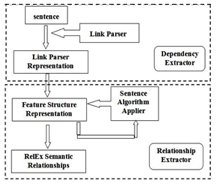
\includegraphics[width=12cm]{figures/RelEx.png}
\protect\caption{\label{fig:relex}Overview of the internal dynamics of the RelEx semantic extraction system, which maps link parses into sets of more abstract syntactico-semantic relationships.}
\end{centering}
\end{figure*}

RelEx的输出可看作是被简化了的输入句子的语法结构,在一定程度上,RelEx还对一些表层关系进行归一化处理,因为很多等效但异构的动词框架会被映射到一致或者同态的特征结构图中。例如下面的两个不同的句子语义却一样:

\begin{verbatim}
      Mary ate the cake.
      The cake was eaten by Mary. 
\end{verbatim}

在RelEx的输出中,它们同时含有下面的RelEx依存关系:

\begin{verbatim}
     _subj(ate, Mary)
     _obj(ate, cake)
\end{verbatim}

\subsection{RelEx的系统框架}{RelEx Framework}

RelEx系统框架主要包括两大模块:附属关系抽取模块和语法关系抽取(参见图\ref{fig:relex})。它能识别句子中词和词之间的主语、宾语、间接宾语和其他依存关系,也能像其他依存语法分析器那样生成依存关系树。 

RelEx首先对句子中的每个词创建一个特征节点(FeatureNode),然后通过一系列相关规则不断更新每个特征节点。这些规则将链语法分析器的输出结果中的不同链的组合转换成相应的RelEx依存关系,有些转换可能是通过某一条规则直接从链到RelEx依存关系的转换,也可能是间接地根据几条规则动态修改一个词的特征节点,并结合其他相关的特征节点中的特征,最终得到相应的RelEx关系。

接下来我们使用在链语法章节中使用的例句“The cat chased a snake.”来更详细地解析RelEx的每个步骤和实现方法。

\noindent {\bf 步骤1:将链语法分析器的输出转换成一个特征结构图。}

如上所述,RelEx首先将链语法分析器的输出结果转换成一个特征结构图。特征结构图是一个带权有向图,其中节点可以表示一个值,也可以是一个无序的特征列表。 RelEx中,特征指的就是一条指向另一个节点的带权边,而特征的值通常是一个字符串。

从上一节中我们可知,例句输入链语法分析器后产生下面的链语法结构: 

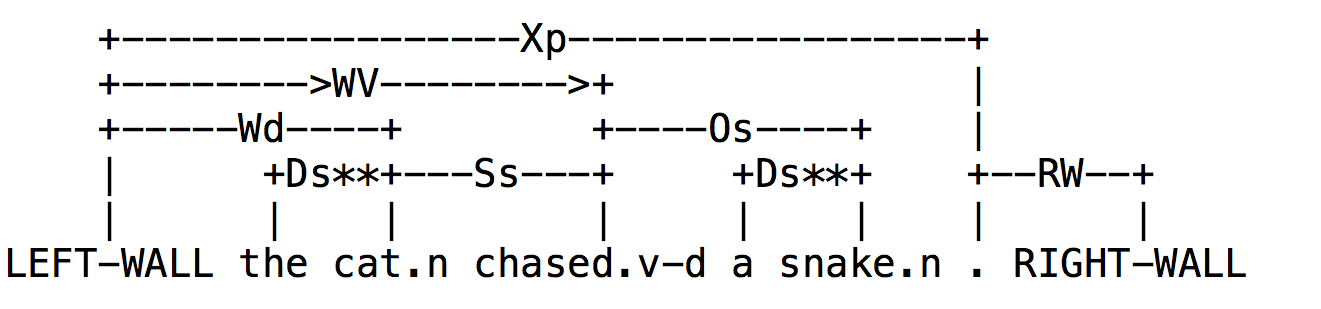
\includegraphics[width=12cm]{figures/catSnake.png}

根据我们上面的步骤描述,首先需要将上面的链语法分析结构转换成特定的特征结构图。句子中的每个词都会被转换成特征结构图的一个节点,其中该节点包含以下特征([]中的内容表示特征的类型,如 NEXT[node]表示该特征是一个特征节点类型):

\begin{itemize}
\item NEXT[node]:该特征指向表示该词的后一个词(如果存在)的特征节点。
\item PREV[node]:该特征指向表示该词的前一个词(如果存在)的特征节点。
\item this[node]:该特征指向自己(该特征的存在只是为了方便某些句子算法的执行)
\item wall[node]:该特征指向表示LEFT-WALL的特征节点。
\item index\_in\_sentence [int]: 该词在句子的位置,LEFT-WALL的位置为0,以此类推。
\item start\_char [int]: 该词的第一个字符在原句子中的位置。从0开始计算。
\item end\_char [int]: 该词的最后一个字符的后一个字符在原句中的位置。 end\_char - start\_char = 字长
\item str [string]: 该词的内容。该内容应该和从句子中取(start\_char, end\_char)之间的子串得到的结果一致。
\item POS [string]: 该词的词性。
\item num\_left\_links [int]: 从该词出发指向左方向的链接个数。
\item num\_right\_links [int]: 从该词出发指向右方向的链接个数。
\item linkL0 [node]: 指向表示从该词出发指向左方向的链接的特征节点
\item linkL(1,2,3,...) [node]: 指向表示从该词出发指向左方向的链接的特征节点(如果从该词出发指向左方向的链接个数超过1)
\item linkR0 [node]: 指向表示从该词出发指向右方向的链接的特征节点
\item linkR(1,2,3,...) [node]: 指向表示从该词出发指向右方向的链接的特征节点(如果从该词出发指向左方向的链接个数超过1)
\end{itemize}

类似地,链语法分析结构中的每个链接也被表示成一个特征节点,其中该节点包含以下特征:

\begin{itemize}
\item LAB [string]: 该链接的名称
\item F\_L[node]: 指向表示该链接左边的词的节点
\item F\_R[node]: 指向表示该链接右边的词的节点
\end{itemize}

\begin{figure}

\begin{centering}
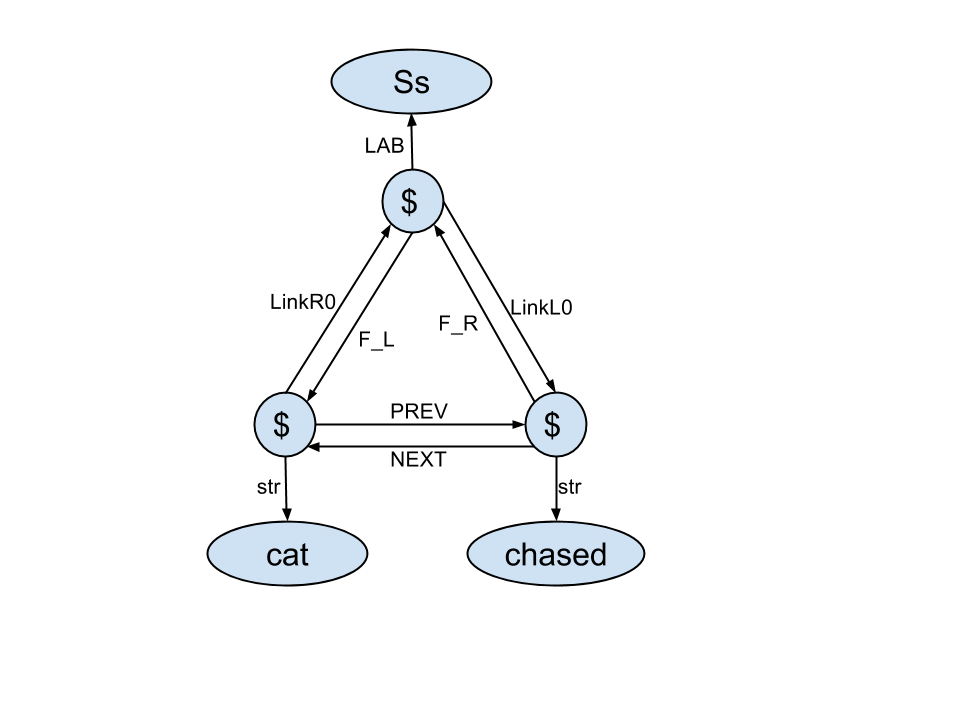
\includegraphics[width=12cm]{figures/featureStructure.png} 
\par\end{centering}

\caption{初始特征结构图\label{fig:featureStructure}}


\end{figure}

不难发现,RelEx中的使用特征结构图非常复杂,为了能更形象地理解特征结构图,本文截取了上述例句的特征结构图的部分来进一步解释(参见图\ref{fig:featureStructure})。
 
  图\ref{fig:featureStructure}中,带\$的节点可以表示代表句子中的某个词的特征节点,通过特征str指向词的内容;也可以表示代表某个链接的特征节点,通过特征LAB指向链接名称。从上图我们可以看出,“cat”和“snake”通过链接Ss相连。例句中的第二个个词节点的特征str表示该词的内容“cat”,特征NEXT指向表示下一个词的特征节点(即str为“chased”的节点),特征F\_L表示该词是链接“Ss”的左右的词。“LinkR0”表示它指向的链接Ss是从该词“cat”出发指向右边的链接。以此类推,不难从上图中找出例句中第三个词节点的一系列相关特征。

\noindent {\bf 步骤2: 执行包含一系列句子算法的句子算法应用器(Sentence Algorithm Applier),对步骤1中得到的特征结构图进行相应的改写操作。}

句子算法应用器从句子算法的定义文件中导入一系列的句子算法,句子算法的执行顺序必须按照定义文件中句子算法的排序。当一个句子算法被执行时,RelEx不断迭代遍历特征结构图中的每一个特征节点,对每个节点都尝试执行该句子算法。句子算法的执行会导致特征结构图的修改,因此它们的操作顺序是很重要的。例如,假如前面的句子算法执行后,特征结构中的所有特征节点的词性(POS)特征都被删除,那么用于处理含有POS特征节点的句子算法将无法被执行。

所有的句子算法都带有一个特定的标记(可以理解成该句子算法的名称),当某个句子算法被成功执行后,该算法会在被成功执行该算法的节点上添加一个特征SIG,并将其赋值为该句子算法名称。被句子算法添加的一个最重要的特征是指向表示词的特征节点的ref,RelEx使用ref特征来输出最后的关系集合。

除了复杂的特征结构,RelEx的另一个核心部分是前文一直提到的句子算法。RelEx使用的句子算法也是很复杂的,可分为抽象的句子算法和需要实例化的句子算法。我们这里选择一个用的最广泛的通用句子算法TemplateActionAlg来进一步阐述。一个TemplateActionAlg实例能接受文本输入,第一行表示该实例的名称(不可重复),接下来是一个用于匹配的模板路径集合(Template Paths和行为路径集合(Action Paths),之间用“=”隔开。对于模板路径\textless x, y, z\textgreater ,表示目标值按照\textless x, y, z\textgreater 这样的路径来解析。对于操作路径\textless x, y, z\textgreater ,表示目标值按照\textless x, y, z\textgreater 这样的路径被赋值。例如,在如下的被实例化的TemplateActionAlg的句子算法中,

\begin{verbatim}
#TemplateActionAlg
SPECIAL-ADJ
; Used for "easy to read." 
; The B links back to the adjective. But it should really be
; interpretted as linking back to the subject of the adjective
<LAB> = \B\.*|\BW\.*
<F_L POS> = adj
=
<F_R obj> = %
<F_R obj> = <F_L subj>
<F_L ADJ-OBJ-FLAG> = T
\end{verbatim}

在该句子算法中,模板就是:

\begin{verbatim}
<LAB> = \B\.*|\BW\.*
<F_L POS> = adj
\end{verbatim}

不难看出,第一行表示用于匹配那些表示链接名称B或者BW的特征节点,句子算法的表示使用了正则表达式,意味着,只要链接名称以B或者BW的特征节点都满足。除此之外,要想上面的句子算法能被执行,还要满足第二行,即该特征节点表示的链接左边的词必须是一个形容词。

如果上面的两条模板都匹配成功,那么下面的操作将会被执行:

\begin{verbatim}
<F_R obj> = %
<F_R obj> = <F_L subj>
<F_L ADJ-OBJ-FLAG> = T
\end{verbatim}

这些操作可被解释如下:第一行的操作表示该链接的右边的词所在的特征节点的obj特征会被清空。清空后,紧接着将该链接左边的词所在的特征节点的sub特征值赋给它。最后,将该链接的左边的词所在的特征节点的ADJ-OBJ-FLAG特征值设为T(真)。

我们接着用上面的例句“The cat chased a snake.”,接下来两个图是图\ref{fig:revisedFeatureStructure}的节选特征结构图,更直观地解释了,通过执行相关的句子算法后,被修改的结构特征图。  
\begin{figure}
\begin{centering}
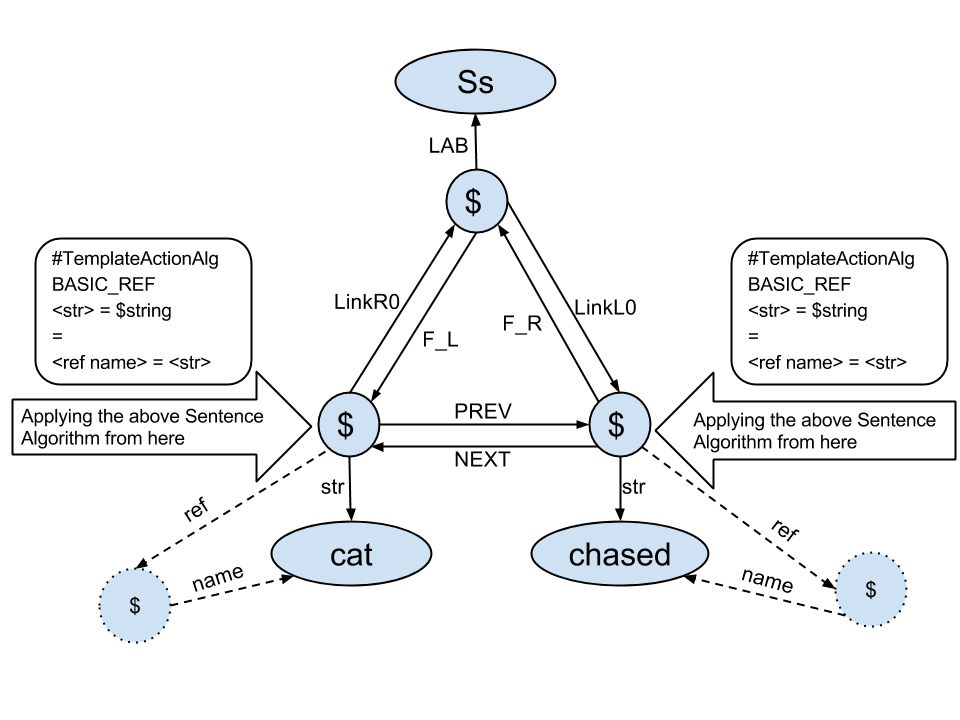
\includegraphics[width=12cm]{figures/revisedFeatureStructure.png} 
\par\end{centering}

\caption{修改过的特征结构图\label{fig:revisedFeatureStructure}}
\end{figure}


图\ref{fig:revisedFeatureStructure}中虚线部分是执行了下面的句子算法后特征结构图被修改的部分:

\begin{verbatim}
#TemplateActionAlg
BASIC_REF
<str> = $string
=
<ref name> = <str>
\end{verbatim}

根据上面的句子算法,当模板“<str> = \$string”被匹配时,会执行操作“<ref name>=<str>”,也就是,把该词的内容赋值给通过路径<ref, name>找到的节点。

\begin{figure}
\begin{centering}
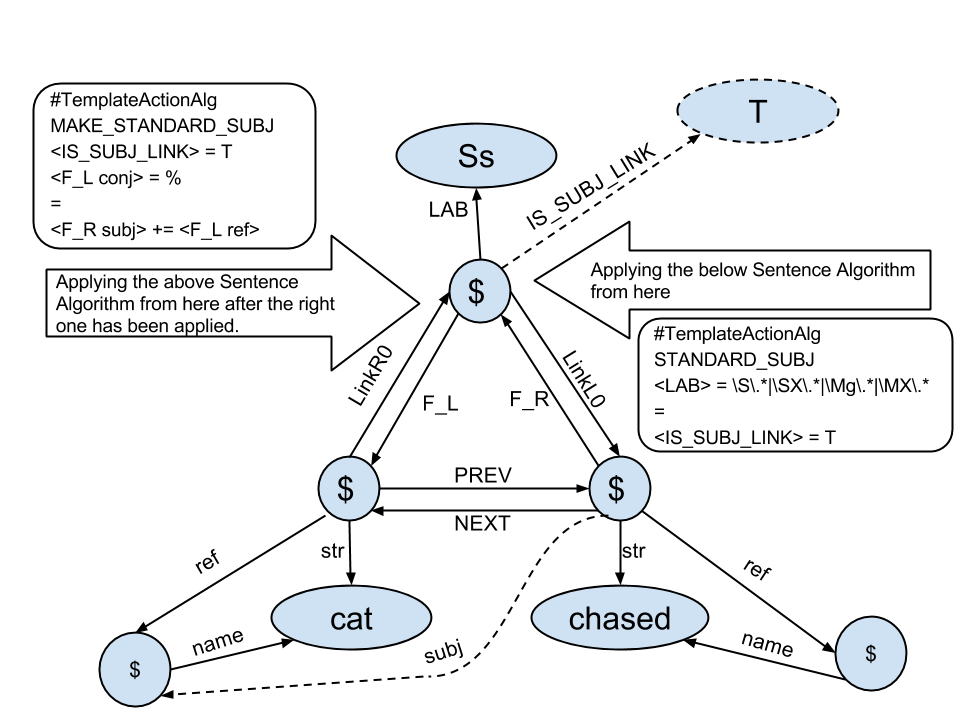
\includegraphics[width=12cm]{figures/revisedFeatureStructure_1.png} 
\par\end{centering}

\caption{修改过的特征结构图\label{fig:revisedFeatureStructure_1}}
\end{figure}

图\ref{fig:revisedFeatureStructure_1}中,同样地,虚线部分表示执行相应的句子算法后特征结构图被修改的部分。其中使用的句子算法有:

\begin{verbatim}
#TemplateActionAlg
STANDARD_SUBJ
<LAB> = \S\.*|\SX\.*|\Mg\.*|\MX\.*
<LAB> != \MX.[rj]\.*
<LAB> != MX|MXs|MXp
=
<IS_SUBJ_LINK> = T
\end{verbatim}

\noindent 如果找到连接主语的链接,那么创建一个名为sub的依存关系:
\begin{verbatim}
#TemplateActionAlg
MAKE_STANDARD_SUBJ
<IS_SUBJ_LINK> = T
<F_L conj> = %
=
<F_R subj> += <F_L ref>
\end{verbatim}

第一个句子算法中表明,当找到一个特征节点的“LAB”特征满足这样的正则表达式 \verb§\S\.*|\SX\.*|\Mg\.*|\MX\.*§时,即图\ref{fig:revisedFeatureStructure_1}中最上面的特征节点的情况,那么会创建一个新的特征IS\_SUBJ\_LINK 并赋值为 "T" (真)。IS\_SUBJ\_LINK 是一个临时特征,会在上面第二个句子算法中用到,类似地,在执行了第一个句子算法后,图中最上面的节点也满足了第二个句子算法的条件,于是会接着执行第二个句子算法,即执行 $<F_R subj> += <F_L ref>$,这说明,系统会将$F_L ref$的值传到通过路径$F_R subj$的相应特征上,也就是上图中最下面的虚线部分显示的。需要说明的是,操作符 "+=" 是指将该操作符右边的值“附加”到通过左边的路径得到的特征上。

\noindent {\bf 步骤3: 遍历最后得到的特征结构图,输出最终的RelEx关系集合。}

当步骤2完成后,我们得到的结构特征图包含了很多RelEx句子算法中使用的临时特征,以及残留的句法特征,因此这一步骤主要是遍历步骤2得到的特征结构图并过滤掉这些不必要的特征,得到最终的简洁直观的RelEx关系树(图),最终抽取其中RelEx的依存关系和词语属性集合并输出。

这里依然采用上面的例句“The cat chased a snake.”。当所有的句子算法都被遍历过后,再过滤掉临时的特征,可以得到一个精简的用于生成RelEx关系集合的特征结构图(图\ref{fig:finalFeatureStructure})。

\begin{figure}
\begin{centering}
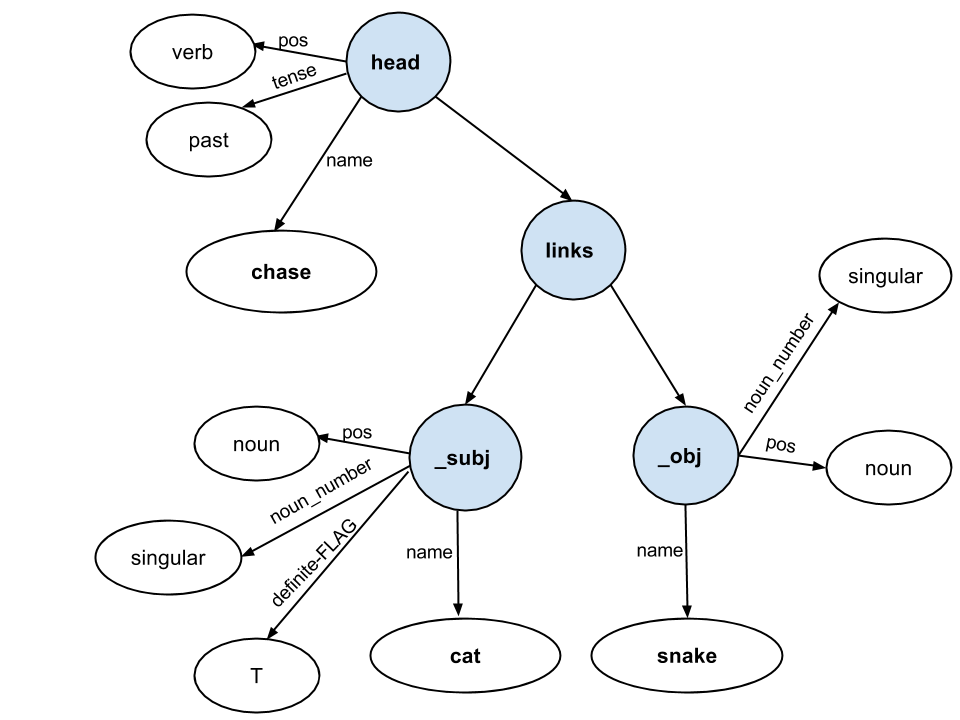
\includegraphics[width=12cm]{figures/finalFeatureStructure.png} 
\par\end{centering}

\caption{最终特征结构图\label{fig:finalFeatureStructure}}

\end{figure}

其中特征节点head指向表示主句或所有从句中的中心词的特征节点。RelEx中与head对应的还有特征节点background(例句中没有),它是指向表示修辞词的节点,如形容词、副词等。

\noindent 根据上图,我们可以从以下的特征节点抽取出每个词的相关属性:
\begin{itemize}
\item name: 指向表示该词的名称的特征节点
\item pos: 指向表示该词的词性标记的特征节点
\item tense: 指向表示该词的时态的特征节点(针对动词)
\item definite-FLAG:指向一个值为“T”的特征节点,表明该名词受量词、定冠词等限定词约束,如“the” "that"等(针对名词)
\item noun\_number: 指向表示该词的单复数形式的特征节点(针对名词)
\end{itemize}

\noindent 类似,可以从以下的特征节点抽取出相关的依存关系:
\begin{itemize}
\item links: 指向表示以该节点为第一参数的依存关系的特征节点
\item \_subj: 指向表示依存关系\_subj(主谓关系)的第二参数的特征节点
\item \_obj: 指向表示依存关系\_obj(动宾关系)的第二参数的特征节点
\end{itemize}

根据图\ref{fig:finalFeatureStructure}中的信息,不难抽取最终的RelEx输出结果:

 \begin{verbatim}
  Dependency relations:

     _obj(chase, snake)
     _subj(chase, cat)

  Attributes:

     tense(chase, past)
     subscript-TAG(chase, .v-d)
     pos(chase, verb)
     pos(., punctuation)
     subscript-TAG(snake, .n)
     pos(snake, noun)
     noun_number(snake, singular)
     definite-FLAG(cat, T)
     subscript-TAG(cat, .n)
     pos(cat, noun)
     noun_number(cat, singular)
     pos(a, det)
     pos(the, det)
\end{verbatim}

其中,依存关系(Dependency relations)可以理解成两个词之间语义角色关系,如主谓关系、动宾关系等 \footnote{RelEx中使用的依存关系类型集合可参见 \url{http://wiki.opencog.org/w/Binary_relations}}。属性(Attributes)是值每个词的词态属性,如词性、时态、人称等 \footnote{RelEx中使用的词态属性集合可参见 \url{http://wiki.opencog.org/w/Word_properties}}。


%%%%%%%%%%%%%%%%%%%%%%%%%%%%%%%%%%%%%%%%%%%%%%%%%%%%%%%%%%%%%%%
\subsection{RelEx关系的形式化}{RelEx Relationship Formalization}
%%%%%%%%%%%%%%%%%%%%%%%%%%%%%%%%%%%%%%%%%%%%%%%%%%%%%%%%%%%%%%%


如前所述,RelEx关系反射了词和词之间的依存关系,如主谓关系、动宾关系、修饰和被修饰关系、所有格关系等等;除此之外,RelEx也同样标注了词的各种词态属性,如时态、词性、单复数等等。为了这些繁琐的关系有一个适合操作以及后续处理的规范体系,本小节提出了一种基于巴克斯范式BNF(Backus Normal Form)的对RelEx关系进行了如下的形式化表示:

 {\tt\begin{scriptsize}\begin{lstlisting}
<RelEx-rel>::== <dependency-rel> | <property-rel>
<dependency-rel>::== <dependency-type> "(" <word-instance> ", " <word-instance>")"
<property-rel> ::== <property-type> "(" <word-instance> ", "<property-value> ")"
<word-instance> ::== <word> <instance> | <word>
  \end{lstlisting}\end{scriptsize}}

其中,

\begin{itemize}
\item RelEx-rel可以是RelEx中的表示两个词之间的依存关系,也可以表示单个词的本身属性和属性值之间的关系。
\item dependency-rel表示RelEx中的依存关系,其中依次包含依存关系类型(即范式中使用的dependency-type),第一参数(一般是单词,有时候也可以是短语)以及第二参数(一般是单词,有时候也可以是短语)
\item property-rel表示RelEx中对词的属性的标注,其中依次包含属性类型(即范式中使用的property-type),词或短语以及属性值。
\item word-instance表示来自所分析的句子中的词,如果同一个词在同一个句子中出现2次或以上,通过在后面加上标记(用整数表示)来区分。
\end{itemize}

%%%%%%%%%%%%%%%%%%%%%%%%%%%%%%%%%%%%%%%%%%%%%%%%%%%%%%%%%%%%%%%
\section{基于涉身的指代消解}{Standard and Embodiment-Based Anaphor Resolution}
%%%%%%%%%%%%%%%%%%%%%%%%%%%%%%%%%%%%%%%%%%%%%%%%%%%%%%%%%%%%%%%

RelEx 含有使用典型 Hobbs 算法实现了简单的指代消解\cite{Hobbs1978}。概括地说,当识别出某语句中的"他"、"她"、"它"等代词,Hobbs 算法就会在近期使用过的语句中进行搜索,并根据数字、性别和其他特征来找出匹配此代词的名词。Hobbs 算法被用来建立一整列以近因排序的候选名词。

一个新的指代消解算法近期已在 OpenCogd的Atomspace中实现,使用了类似Hobbs算法中指代消解的解决思路,但是使用了更灵活的知识表示,也能结合语义链接。本文实现了此算法,让一个以 OpenCog 控制的智能体生活在充斥着物体的环境,而每个物体都有它们自己的特性。此范例采用的是当前以 Atomspace 为基础、但较早期版本的指代消解系统,而有一段视频描述了这个范例\url{https://www.youtube.com/watch?v=ii-qdubNsx0)}。

举例来说,在一游戏世界中,我们可以有许多各种颜色和大小的球。我们运用多个节点将此呈现在 OpenCog Atomspace:表示"球"的概念的单个 ConceptNode、与"球"相关联的一个 WordNode、以及表示特定球的多个 ConceptNode。当然有些 ConceptNode 也表达其他与球有关的概念,像是"又鼓又大、会发出咯吱声的球"、"可用球棒挥击的球"等不概述于任何自然语言字词的概念。

当智能体与世界互动时,它会通过感知来学到寻获物体的相关信息。关联某设定物体的感知会贮存为其他表示特定物体实例的节点。所有此信息会使用RelEx2Logic 被呈现在 Atomspace 之中(这部分在下一节会举例说明)。

举例来说,当用户说"抓红色的球"( ”Grab the red ball”),智能体就必须理解用户指的是那种球 – 例如它必须唤起参照消解程序。参照消解使用句中的信息来选择物件、和些许捷思规则。概括而言,参照消解是根据智能体通过感知获取关于世界的知识,将用户句中的名词对应到虚拟世界的实际物体。

在这个例子中,首先智能体会选择相关"球"字眼的 ConceptNode,再利用句中的决定因素和其他适当的限制条件,检验所有与这些概念关联的个别实例(就此范例而已,决定因素为形容词"红色";而由于动词为"抓",因此它也会寻找可抓取的物体)。若它找到不止一个"可抓取的红球",就会使用捷思规则来选取一个(在这个情况,智能体会选择离自己最近的物体)。

智能体也须将句中的代词对应到虚拟世界的实际物体。例如,若用户说"我喜欢红色的球。抓起它"(”I like the red ball. Grab it”),智能体就必须将代词"它"(”it”) 对应到特定的红球。此程序分两个阶段执行:首先使用指代消解将代词"它"(”it”) 与先前听到的名词"球"(”ball”) 联系;接着使用参照消解将名词"球"(”ball”) 与实际物体联系在一起。

在此情境中,我们可使用智能体对世界的知识改良 Hobbs 演算的结果,以帮助选出最佳的候选名词。假设智能体听到这些句子:


\begin{verbatim}
"球是红色的。"("The ball is red.")
"棍子是棕色的。"("The stick is brown.") 

\end{verbatim}

\noindent and then it receives a third sentence

\begin{verbatim}
"抓它。"("Grab it.")
\end{verbatim}

指代消解器将构建一个列表,此列表包含针对第三个句子中代词“it”的两个选项:ball和stick。如果stick是最近使用的名词,那么正如Hobbs建议的那样,代理将抓取stick,而不是ball。

与此类似,如果智能体的历史包含

\begin{verbatim}
"From here I can see a tree and a ball."
"Grab it."
\end{verbatim}

那么Hobbs的算法按顺序返回名词tree和ball作为候选。但是如果使用我们的集成的指代消解处理,智能体将推断不能抓取tree,所以仅选择ball。


%%%%%%%%%%%%%%%%%%%%%%%%%%%%%%%%%%%%%%%%%%%%%%%%%%%%%%%%%%%%%%%
\section{RelEx2Logic:逻辑关系抽取}{RelEx2Logic: Translating Linguistic Dependency Relations into Logical Relations}
%%%%%%%%%%%%%%%%%%%%%%%%%%%%%%%%%%%%%%%%%%%%%%%%%%%%%%%%%%%%%%%

本章节介绍我们的自然语言理解系统中最后的纯语言学阶段,即RelEx2Logic。RelEx2Logic是我们本文工作的一个关键组成部分,用于将RelEx生成的句法-语义关系转换成PLN和其它OpenCog认知组件可以使用的基于超图的逻辑表示形式,从而使得我们的自然语言理解系统可以与逻辑推理系统(例如PLN)、控制系统(例如OpenPsi)和OpenCog的其它组件进行有效交互。

\subsection{RelEx2Logic}{RelEx2Logic}

众所周知,自然语言的逻辑极其复杂,而且即使在给定的表示形式下,同一个句子可以用很多种不同的逻辑表达方式,而不影响该句子想要表达的语义。因此在我们的工作中,即通过OpenCog中的Atomspace来表示自然语言的语义关系和结构,必须面对这个事实:即使对于一个简单地句子,也可以有很多种不同结构的基于Atomspace的逻辑形式来相同或等价的语义。RelEx2Logic系统的目标是以尽可能简单的方式将RelEx输出映射到PLN可以理解和推理的AtomSpace表示,生成可以获取相关表达所包含的大量含义的精确表示。RelEx2Logic不会试图消解RelEx输出中所有的语义歧义,而是专注于将这些语义歧义表达成一种易于发现和处理的方式,这样能使这些歧义义在整个认知体系结构的知识库上或者借助涉身相关的信息,通过简单的常识推理而得到解决。

具体实现上,RelEx2Logic的核心理念是通过应用一系列简单的重写规则以及较复杂的后处理规则(处理复杂句子和问题需要这些后处理规则,例如进行概念实例区分)把RelEx关系映射到语义解释(例如OpenCog的AtomSpace表示)。

每个核心重写规则的输入是句法分析图中满足特定约束的子图,输出是一个原子(Atom)超图。在实践中,需要的规则通常采用成对标记(G,A)的形式,其中:

\begin{itemize}
\item $G$是一个图,其节点是单词或变量,其边是RelEx关系类型。
\item  $A$是一个超图,其节点是单词、变量或特殊的语言学节点(根据一个小型词汇表绘制),其超图链接是OpenCog原子(Atom)类型(例如InheritanceLink和EvaluationLink)。
\item $G$和$A$中的变量列表必须相同。
\end{itemize}

我们把符合这种说明的规则称为“简单映射规则”。

对于处理人类语言真正需要的简单映射规则来讲,满足约束条件{\bf $G$中的每个边映射到$A$中的单个超图链接}。从数学上讲,这个约束条件的后半部分意味着每个重写规则各自都是一个图同态\cite{Voloshin2009},这进一步意味着一起应用的一系列重写规则也是一个图同态。

这种规则的一个简单例子是这样一个(G,A),其中
$$
G = \{ S_*(v_1,v_2), \ O_*(v_1, v_3) \}
$$

$$
A = (EvaluationLink \ v_1 \ v_2 \ v_3)
$$

这把主语为$v_2$,宾语为$v_3$的动词$v_1$映射到一个v1为谓语,($v_2$, $v_3$)为参数列表的OpenCog EvaluationLink。例如,$S_*$ 指任何$S$的链路分析器子类型。当然,大部分规则都比这个例子复杂。

在具体操作中,由于自然语言的复杂性,仍然有一些这种形式的RelEx2Logic规则无法处理的语言现象。所以,为了获取句子正确的逻辑表示而不影响其含义,我们向RelEx2Logic框架添加一个后处理步骤,这个步骤主要包含下列部分:

\begin{itemize}
\item 处理OpenCog Atomspace中的实例。根据输入的自然语言的含义,将通用概念或谓语与特定概念或谓语进行区分。
\item 估计模糊谓语或概念的概率。例如,如果句子是“Maybe the cat chased a snake.”,那么我们需要给最后的逻辑表示指定相较于句子“the cat chased a snake.”较低的概率。
\item 正确处理量词。众所周知,自然语言中的量词十分复杂。不可能创建一个通用规则而以通用方式获取所有量词的正确抽象表示。而且,我们想要使得我们的规则更加通用,所以我们不想为每个量词使用单独的规则,这需要以简化的方式编写量词规则,而不是极力利用后处理方法允许的更大灵活性。
\end{itemize}

下面将解释后处理的更多细节。

将我们当前的简单映射规则应用于上述的例句“The cat chased a snake.”,会生成以下基本输出:

 {\tt\begin{small}\begin{lstlisting}
EvaluationLink 
      PredicateNode chase@3453432
      ListLink
            ConceptNode cat@1243546464
            ConceptNode snake@564636322
       
\end{lstlisting}\end{small}}

这些“基本输出”仅仅是这个句子解释后Atomspace中所创建的完整原子(Atom)集合的一小部分。一个更完整的列表是

{\tt\begin{small}\begin{lstlisting}
((ReferenceLink
   (InterpretationNode "sentence@f207bfb1-8dcf-42c8-a1d7-9d89075e8be8_parse_0_interpretation_$X")
   (SetLink
      (ImplicationLink
         (PredicateNode "chased@64f680a3-d076-4ae1-814c-0152c3f3c8f8")
         (PredicateNode "chase" (ptv 1 0 1))
      )
      (InheritanceLink
         (ConceptNode "cat@3a186cb8-f8e2-40b1-97fc-525d51d29f57")
         (ConceptNode "cat" (ptv 1 0 1))
      )
      (InheritanceLink
         (ConceptNode "snake@b8aabaee-dfe9-4833-8b89-6d9c1d45aea0")
         (ConceptNode "snake" (ptv 1 0 1))
      )
      (EvaluationLink
         (PredicateNode "chased@64f680a3-d076-4ae1-814c-0152c3f3c8f8")
         (ListLink
            (ConceptNode "cat@3a186cb8-f8e2-40b1-97fc-525d51d29f57")
            (ConceptNode "snake@b8aabaee-dfe9-4833-8b89-6d9c1d45aea0")
         )
      )
      (InheritanceLink
         (PredicateNode "chased@64f680a3-d076-4ae1-814c-0152c3f3c8f8")
         (ConceptNode "past")
      )
      (InheritanceLink
         (InterpretationNode "sentence@f207bfb1-8dcf-42c8-a1d7-9d89075e8be8_parse_0_interpretation_$X")
         (ConceptNode "DeclarativeSpeechAct")
      )
      (EvaluationLink
         (PredicateNode "definite")
         (ListLink
            (ConceptNode "cat@3a186cb8-f8e2-40b1-97fc-525d51d29f57")
         )
      )
   )
)
\end{lstlisting}\end{small}}

本节最后会给出更多映射例子以及所涉及原子(Atom)类型的解释。

如果链路分析器给出多个分析选项,RelEx2Logic规则将为每个分析选项提供一个逻辑解释。目前已经实现基于语料库进行统计启发来排列多个分析的可信性,当然这并不完美。一些情况中,会向OpenCog提供多个逻辑输出选项,并且必须基于更高层次的上下文推断在这些选项之间进行选择,这是当前研究的一个难题和主题。


\subsection{RelEx2Logic所使用的规则}{RelEx2Logic Rules}

为了将RelEx关系转换成抽象的OpenCog AtomSpace逻辑表示,我们引入一系列RelEx2Logic规则。RelEx2Logic规则(以前称为Link2Atom和Syn2Sem规则\cite{Lian2012})是一系列人工编码的规则,用于把RelEx的输出映射到OpenCog原子(Atom)表示的形式,这种表示更适合于由PLN和其它工具进行自动化推断。本节总结性地阐述规则集合并给出一些规则例子。可以在\url{opencog/nlp/scm/relex-to-logic.scm}在线找到所有规则。

RelEx2Logic规则有多个目标:

\begin{itemize}
\item 作为运行的OpenCog自然语言处理系统的一部分,其潜在用途包括文本分析和自然语言对话。
\item 作为概念研究工具,帮助我们理解句法-语义输出(例如RelEx生成的句法-语义输出)映射到更抽象的逻辑关系(例如PLN采用的逻辑关系)的问题。
\item 作为工具来帮助生成成对(链路分析和抽象的PLN形式的原子)的语料库,然后可以自动分析此语料库来产生语言理解和生成规则(更多信息请参见Syn2Sem)。
\end{itemize}

{\bf 示例规则(Tense规则)}

为了方便阐述剩下的内容,我们从一个非常简单的RelEx2Logic规则例子开始。当然,大部分规则比这个例子复杂。此处,为了方便人理解,采用RelEx SFF格式(RelEx许多输出格式中的一种)来说明规则输入。

为了用便于阅读的方式说明RelEx2Logic规则,我们在此使用类似以下的格式:

\begin{verbatim}
规则输入:
tense(W, Tense)
pos(W, verb)
规则输出:
(tense-rule W (get_instance_name W word_index sentence_index) Tense)
\end{verbatim}

在OpenCog中运行此规则,规则的输出将启动一个帮助函数(helper function,用Scheme语言编写)。下面会列出这个帮助函数。然后帮助函数将最终生成最后的OpenCog Atomspace表示。

如同上一小节中所述,在我们软件实现中,我们使用诸如(ImplicationLink $P_G$ $P_A$)这样的格式来表示RelEx2Logic规则,从而使得RelEx2Logic与OpenCog系统的其余组件保持一致。例如,这种格式意味着规则可以由OpenCog模式匹配器来执行(OpenCog模式匹配器用来在OpenCog Atomspace中搜索原子的特定模式、排列或“模板”)。所以上述简单的RelEx2Logic规则在当前系统中将被如下表示:

\begin{verbatim}
ImplicationLink
     EvaluationLink
           PredicateNode "tense"
           ListLink
                WordNode W
                ConceptNode Tense
     ExecutionOutputLink
              GroundedSchemNode "r2l/tense-rule.scm"
              ListLink
                   WordNode W
                   ConceptNode Tense
                   NumberNode word_index
                   NumberNode sentence_index

\end{verbatim}

对应于上述RelEx2Logic规则的提供后处理的相应帮助函数为:

\begin{verbatim}
帮助函数:
(define (tense-rule verb instance tense)
   (define new_predicate (PredicateNode instance))
   (define verb_node (PredicateNode verb)) 
   (define tense_node (ConceptNode tense))
   (list
      (InheritanceLink new_predicate verb_node)
      (InheritanceLink new_predicate tense_node)
   )
)

例子:
tense(chase, Past)
pos(chase, verb)
==>
(tense-rule "chase" "chase@3453432" "Past")
==>
(InheritanceLink "chase@3453432" chase)
(InheritanceLink "chase@3453432" Past)

\end{verbatim}

注意:这个例子使用了额外的帮助函数$get\_instance\_name$。

下面解释这个帮助函数。本质上,这个函数只是为概念的实例选择一个在给出的AtomSpace中唯一的名字(例如,它可能为$chair$的实例选择名字$chair77$)。如果单词W在句子中是第K次出现,那么单词序号为K。句子序号是该句子区别于其它句子的一个标识符。

\subsection{RelEx2Logic的后处理过程}{PostProcessing}

RelEx2Logic最初的设计意图是如同上述例子那样通过直接的逻辑含义进行所有需要的处理。但是随着工作的进展,我们认识到这样做在许多情况中会非常麻烦,同时我们发现引入一些更精巧的后处理方法是最直接的解决办法。此处我们阐述这些后处理规则的基本类型。

现阶段,我们已经实现的后处理规则包括下列类别:

\begin{itemize}
\item 量词:为带有量词的单词引入变量并通过使用相应的链路限定变量的范围,同时给链路指定一些真值。
\item 模糊情态动词:为模糊情态动词发生过修改的谓语指定一些置信下限。例如“Maybe dogs like fish.”,这表示“dogs like fish”的置信度不是很高,所以我们把“he is a genius.”的置信度从默认的0.99调整为0.5。
\item 冗余实例清理:为可以从句法分析知道的通用概念清理实例号。例如“Dogs like meat.”,没有为dogs和meat指定任何明确的冠词、修饰语或代词,并且也没有意指任何其它概念,所以我们认为dogs和meat指通用概念dog和meat,而不是某些特定概念(特定概念需要指定实例号)。
\end{itemize}

下面更详细地阐述我们怎样为上面列出的每种类别实现后处理。

{\bf 量词:}在前面的阶段,我们使用量词记号来标记需要进行后处理的量词。例如“All dogs like meat.”,在应用量词RelEx2Logic规则期间创建“allmarker”并生成下列结果。

\begin{verbatim}
           EvaluationLink
                 PredicateNode "allmarker"
                  ListLink
                         ConceptNode "dog@13456"
\end{verbatim}

本例中,在后处理阶段,我们为量词“all”引入“ForAllLink”(它代表OpenCog Atomspace中的通用量化)和变量节点“\$X”来限定范围包含所有含有$dog@13456$的链路。然后,每个$dog@13456$都将被替换为VariableNode “\$X”。“allmarker”将在后处理后被删除。所以,在后处理结束后,将创建:

\begin{verbatim}
           ForAllLink
                 VariableNode "$X"
                 ImplicationLink 
                        InheritanceLink "$X" noun_instance
                        AndLink
                            ** links involving "dog@13456" **
\end{verbatim}

{\bf 模糊情态动词:}模糊情态动词后处理类似于量词后处理,我们在应用相关的RelEx2Logic规则期间使用相应的记号来标记模糊情态动词。例如,对于句子“Maybe dogs like fish.”,在应用Maybe RelEx2Logic规则后生成下列表示:

\begin{verbatim}
           EvaluationLink
                  PredicateNode "maybemarker"
                  ListLink
                        PredicateNode "like@9768"
\end{verbatim}

然后,用于后处理的$maybemarker$帮助函数将查找所有包含“like@9768”的根链路,并将置信度从默认的0.99调整为0.5。

{\bf 冗余实例清理:}因为不想在句子转换成抽象语义表示期间丢失任何来自句法层面的信息,我们在后处理阶段设立“实例清理”步骤。在当前方法中,我们为句子中每个非组合单词创建一个单独的实例节点。但是,在很多情况中,这会生成许多不必要的实例节点。例如,在句子“Dogs like yummy meat.”中,无需创建诸如$yummy@1765$和$dog@2593$的实例节点,因为这个句子没有指定特定的“dog”和特殊的“yummy”。所以只创建类似以下的链路就已足够:

\begin{verbatim}
         InheritanceLink 
                  ConceptNode   "meat@3976" 
                  ConceptNode   "yummy"

         EvaluationLink 
                  PredicateNode "like"
                  ListLink
                       ConceptNode "dog"
                       ConceptNode "meat@3976"
\end{verbatim}

但是,一个诸如“meat@3976”的实例节点更加有用。因为在这个句子中,它仅陈述“Dogs like ’YUMMY’ meat”,而并非一般的“meat”。

要想知道哪些单词真正需要实例节点,必须在一定程度上理解句子的结构。当前,我们使用一些常识性的规则开始这个过程。确切地讲,如果一个单词没有被修改(名词被形容词修改或者动词被副词修改),或者没有被定冠词限定,或者使用代词,那么此单词的实例节点为“冗余”。清理实例的后处理进行以下工作:

\begin{itemize}
\item 在Atomspace中(或者仅在RelEx2Logic规则的本地输出中)检查是否存在任何此名字的原子为“冗余”。
\item 如果找到冗余原子,那么将其删除并将它的链路移至其父概念。
\end{itemize}
%%%%%%%%%%%%%%%%%

%%%%%%%%%%%%%%%%%%%%%%%%%%%%%%%%%%%%%%%%%%%%%%%%%%%%%%%%%%%%%%%
\section{实验结果举例}{Examples and Analysis}  
%%%%%%%%%%%%%%%%%%%%%%%%%%%%%%%%%%%%%%%%%%%%%%%%%%%%%%%%%%%%%%%

本节中给出更多例子来解释我们的语言理解的理解管道,包含前面阐述的所有部分:Link Parser、RelEx和RelEx2Logic。在后面的章节中,这些特定例子也会在下一章中用来阐述基于自然语言的推理。


\noindent {\bf 例1:Socrates is a man.}

{\bf 链语法分析器输出:}

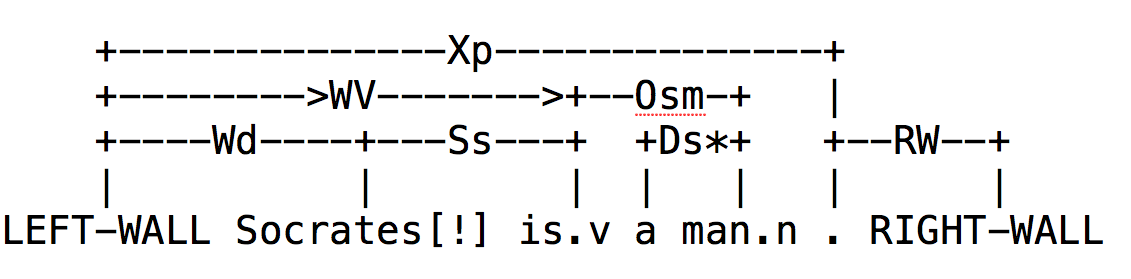
\includegraphics[width=12cm]{figures/Socrates_1.png}

{\bf RelEx输出:}

\begin{verbatim}
Dependcy Relations:

    _obj(be, man)
    _subj(be, Socrates)

Attributes:

    tense(be, present)
    subscript-TAG(be, .v)
    pos(be, verb)
    pos(., punctuation)
    subscript-TAG(man, .n)
    pos(man, noun)
    noun_number(man, singular)
    definite-FLAG(Socrates, T)
    pos(Socrates, noun)
    noun_number(Socrates, singular)
    pos(a, det)

\end{verbatim}

{\bf RelEx2Logic输出:}

 {\tt\begin{small}\begin{lstlisting}
((ReferenceLink
   (InterpretationNode "sentence@f04de205-0f67-471d-84fc-2f9c6103ebca_parse_0_interpretation_$X")
   (SetLink
      (InheritanceLink
         (ConceptNode "Socrates@cfbb87d6-5444-4845-a673-8d70b93ffde6")
         (ConceptNode "Socrates" (ptv 1 0 1))
      )
      (InheritanceLink
         (ConceptNode "man@fe411437-7607-4169-abcf-d42ebcd50338")
         (ConceptNode "man" (ptv 1 0 1))
      )
      (InheritanceLink
         (ConceptNode "Socrates@cfbb87d6-5444-4845-a673-8d70b93ffde6")
         (ConceptNode "man@fe411437-7607-4169-abcf-d42ebcd50338")
      )
      (ImplicationLink
         (PredicateNode "is@b06a386e-0983-4bc8-bd1e-395b487faff2")
         (PredicateNode "be" (ptv 1 0 1))
      )
      (InheritanceLink
         (PredicateNode "is@b06a386e-0983-4bc8-bd1e-395b487faff2")
         (ConceptNode "present")
      )
      (InheritanceLink
         (InterpretationNode "sentence@f04de205-0f67-471d-84fc-2f9c6103ebca_parse_0_interpretation_$X")
         (ConceptNode "DeclarativeSpeechAct")
      )
      (EvaluationLink
         (PredicateNode "definite")
         (ListLink
            (ConceptNode "Socrates@cfbb87d6-5444-4845-a673-8d70b93ffde6")
         )
      )
   )
)
)
\end{lstlisting}\end{small}}


\noindent {\bf 例2: } Men breathe air.

{\bf 链语法分析器输出:}

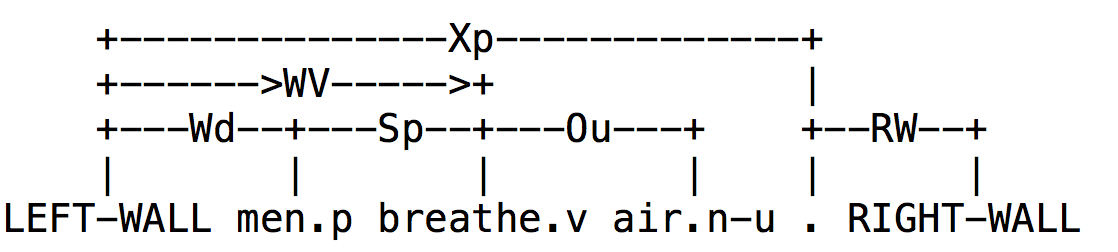
\includegraphics[width=12cm]{figures/Socrates_2.png}


{\bf RelEx输出:}

\begin{verbatim}

Dependcy Relations:

    _obj(breathe, air)
    _subj(breathe, man)

Attributes:

    tense(breathe, present)
    subscript-TAG(breathe, .v)
    pos(breathe, verb)
    pos(., punctuation)
    subscript-TAG(air, .n-u)
    pos(air, noun)
    noun_number(air, uncountable)
    subscript-TAG(man, .p)
    pos(man, noun)
    noun_number(man, plural)

\end{verbatim}

{\bf RelEx2Logic输出:}

{\tt\begin{small}\begin{lstlisting}
((ReferenceLink
   (InterpretationNode "sentence@05b9ba83-e424-43c8-b5f1-8261217bc548_parse_0_interpretation_$X")
   (SetLink
      (ImplicationLink
         (PredicateNode "breathe@ba9dec0b-b99f-4c2c-a5cc-31cc9aa4f172")
         (PredicateNode "breathe" (ptv 1 0 1))
      )
      (InheritanceLink
         (ConceptNode "men@5f6e723d-e57e-47e5-89df-ee9daaa2936d")
         (ConceptNode "man" (ptv 1 0 2))
      )
      (InheritanceLink
         (ConceptNode "air@98afd45c-4807-4607-a732-298c7979327f")
         (ConceptNode "air" (ptv 1 0 1))
      )
      (EvaluationLink
         (PredicateNode "breathe@ba9dec0b-b99f-4c2c-a5cc-31cc9aa4f172")
         (ListLink
            (ConceptNode "men@5f6e723d-e57e-47e5-89df-ee9daaa2936d")
            (ConceptNode "air@98afd45c-4807-4607-a732-298c7979327f")
         )
      )
      (InheritanceLink
         (PredicateNode "breathe@ba9dec0b-b99f-4c2c-a5cc-31cc9aa4f172")
         (ConceptNode "present")
      )
      (InheritanceLink
         (InterpretationNode "sentence@05b9ba83-e424-43c8-b5f1-8261217bc548_parse_0_interpretation_$X")
         (ConceptNode "DeclarativeSpeechAct")
      )
   )
)
)
\end{lstlisting}\end{small}}

\noindent {\bf 例3: }  Socrates breathes air.

{\bf 链语法分析器输出:}

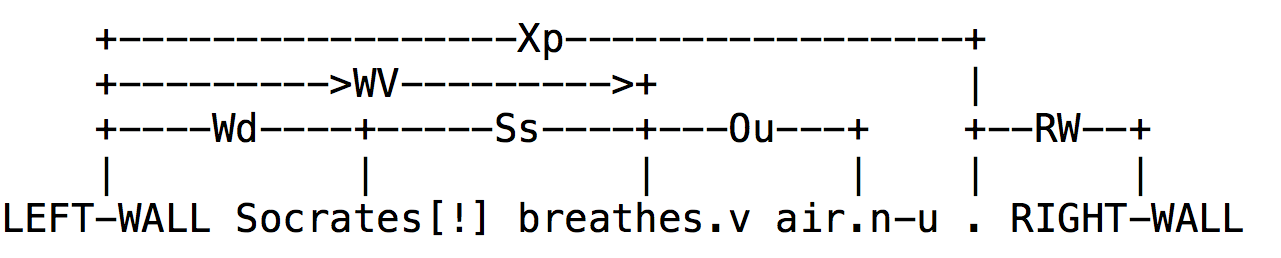
\includegraphics[width=12cm]{figures/Socrates_3.png}

{\bf RelEx输出:}

\begin{verbatim}

Dependcy Relations:

    _obj(breathe, air)
    _subj(breathe, Socrates)

Attributes:

    tense(breathe, present)
    subscript-TAG(breathe, .v)
    pos(breathe, verb)
    pos(., punctuation)
    subscript-TAG(air, .n-u)
    pos(air, noun)
    noun_number(air, uncountable)
    definite-FLAG(Socrates, T)
    pos(Socrates, noun)
    noun_number(Socrates, singular)

\end{verbatim}

{\bf RelEx2Logic输出:}

{\tt\begin{small}\begin{lstlisting}
((ReferenceLink
   (InterpretationNode "sentence@a41e5f83-4a87-4c3f-ad39-833510272d90_parse_0_interpretation_$X")
   (SetLink
      (ImplicationLink
         (PredicateNode "breathes@0a04573a-c867-458d-baa9-0f347ee73371")
         (PredicateNode "breathe" (ptv 1 0 2))
      )
      (InheritanceLink
         (ConceptNode "Socrates@a34bbdf7-1dac-4e62-9dfa-48e1a1f9710c")
         (ConceptNode "Socrates" (ptv 1 0 2))
      )
      (InheritanceLink
         (ConceptNode "air@016cb5c7-35b7-42c4-8690-e3958030773f")
         (ConceptNode "air" (ptv 1 0 2))
      )
      (EvaluationLink
         (PredicateNode "breathes@0a04573a-c867-458d-baa9-0f347ee73371")
         (ListLink
            (ConceptNode "Socrates@a34bbdf7-1dac-4e62-9dfa-48e1a1f9710c")
            (ConceptNode "air@016cb5c7-35b7-42c4-8690-e3958030773f")
         )
      )
      (InheritanceLink
         (PredicateNode "breathes@0a04573a-c867-458d-baa9-0f347ee73371")
         (ConceptNode "present")
      )
      (InheritanceLink
         (InterpretationNode "sentence@a41e5f83-4a87-4c3f-ad39-833510272d90_parse_0_interpretation_$X")
         (ConceptNode "DeclarativeSpeechAct")
      )
      (EvaluationLink
         (PredicateNode "definite")
         (ListLink
            (ConceptNode "Socrates@a34bbdf7-1dac-4e62-9dfa-48e1a1f9710c")
         )
      )
   )
)
)
\end{lstlisting}\end{small}}

\noindent {\bf 例4: }  I think Socrates is a man.

{\bf 链语法分析器输出:}

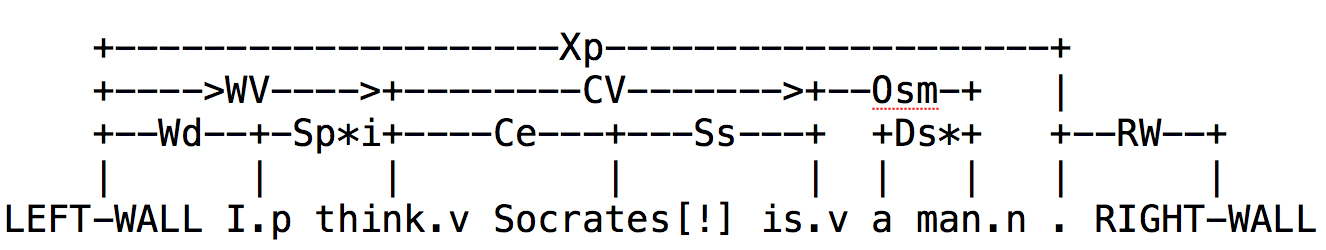
\includegraphics[width=12cm]{figures/Socrates_4.png}

{\bf RelEx输出:}

\begin{verbatim}

Dependcy Relations:

    _obj(be, man)
    _subj(be, Socrates)
    _rep(think, be)
    _subj(think, I)

Attributes:

    definite-FLAG(Socrates, T)
    pos(Socrates, noun)
    noun_number(Socrates, singular)
    pos(., punctuation)
    subscript-TAG(man, .n)
    pos(man, noun)
    noun_number(man, singular)
    pos(a, det)
    tense(be, present)
    HYP(be, T)
    subscript-TAG(be, .v)
    pos(be, verb)
    tense(think, present)
    subscript-TAG(think, .v)
    pos(think, verb)
    pronoun-FLAG(I, T)
    gender(I, person)
    definite-FLAG(I, T)
    subscript-TAG(I, .p)
    pos(I, noun)
    noun_number(I, singular)

\end{verbatim}

{\bf RelEx2Logic输出:}

 {\tt\begin{small}\begin{lstlisting}

((ReferenceLink
   (InterpretationNode "sentence@ec1ca4d5-20ce-465c-9686-aa3edd4dbb2f_parse_0_interpretation_$X")
   (SetLink
      (ImplicationLink
         (PredicateNode "think@8be218e8-095b-44e7-b321-ee877fe4ad45")
         (PredicateNode "think" (ptv 1 0 1))
      )
      (InheritanceLink
         (ConceptNode "I@8c841336-dc92-4c3a-a5af-2e860365ff88")
         (ConceptNode "I" (ptv 1 0 1))
      )
      (EvaluationLink
         (PredicateNode "think@8be218e8-095b-44e7-b321-ee877fe4ad45")
         (ListLink
            (ConceptNode "I@8c841336-dc92-4c3a-a5af-2e860365ff88")
         )
      )
      (ImplicationLink
         (PredicateNode "is@14df1d2f-f71e-45c9-b4a3-80eb38c6a89f")
         (PredicateNode "be" (ptv 1 0 2))
      )
      (EvaluationLink
         (PredicateNode "think@8be218e8-095b-44e7-b321-ee877fe4ad45")
         (ListLink
            (ConceptNode "is@14df1d2f-f71e-45c9-b4a3-80eb38c6a89f")
         )
      )
      (InheritanceLink
         (PredicateNode "think@8be218e8-095b-44e7-b321-ee877fe4ad45")
         (ConceptNode "present")
      )
      (InheritanceLink
         (ConceptNode "Socrates@c1fde686-ae83-45e8-a60d-259179597e68")
         (ConceptNode "Socrates" (ptv 1 0 3))
      )
      (EvaluationLink
         (PredicateNode "definite")
         (ListLink
            (ConceptNode "Socrates@c1fde686-ae83-45e8-a60d-259179597e68")
         )
      )
      (InheritanceLink
         (InterpretationNode "sentence@ec1ca4d5-20ce-465c-9686-aa3edd4dbb2f_parse_0_interpretation_$X")
         (ConceptNode "DeclarativeSpeechAct")
      )
      (InheritanceLink
         (ConceptNode "man@aed74351-8482-4a5b-a6f4-3e979b537fae")
         (ConceptNode "man" (ptv 1 0 3))
      )
      (InheritanceLink
         (ConceptNode "Socrates@c1fde686-ae83-45e8-a60d-259179597e68")
         (ConceptNode "man@aed74351-8482-4a5b-a6f4-3e979b537fae")
      )
      (InheritanceLink
         (PredicateNode "is@14df1d2f-f71e-45c9-b4a3-80eb38c6a89f")
         (ConceptNode "present")
      )
      (EvaluationLink
         (PredicateNode "definite")
         (ListLink
            (ConceptNode "I@8c841336-dc92-4c3a-a5af-2e860365ff88")
         )
      )
   )
)
)
\end{lstlisting}\end{small}}

\noindent {\bf 例5: }  Bob thinks Socrates is a woman.

{\bf 链语法分析器输出:}

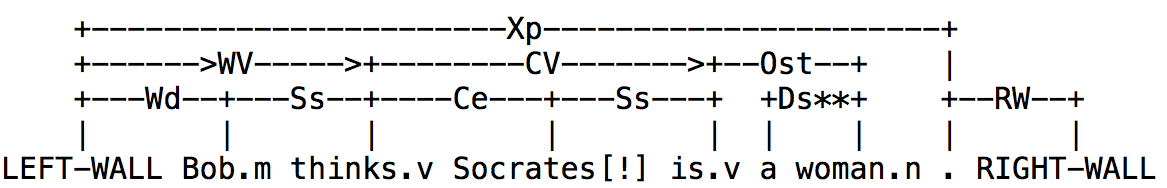
\includegraphics[width=12cm]{figures/Socrates_5.png}

{\bf RelEx输出:}

\begin{verbatim}

dependcy Relations:

    _obj(be, woman)
    _subj(be, Socrates)
    _rep(think, be)
    _subj(think, Bob)

Attributes:

    definite-FLAG(Socrates, T)
    pos(Socrates, noun)
    noun_number(Socrates, singular)
    pos(., punctuation)
    subscript-TAG(woman, .n)
    pos(woman, noun)
    noun_number(woman, singular)
    pos(a, det)
    tense(be, present)
    HYP(be, T)
    subscript-TAG(be, .v)
    pos(be, verb)
    tense(think, present)
    subscript-TAG(think, .v)
    pos(think, verb)
    gender(Bob, masculine)
    definite-FLAG(Bob, T)
    person-FLAG(Bob, T)
    subscript-TAG(Bob, .m)
    pos(Bob, noun)
    noun_number(Bob, singular)

\end{verbatim}

{\bf RelEx2Logic输出:}

 {\tt\begin{small}\begin{lstlisting}

((ReferenceLink
   (InterpretationNode "sentence@8c6d9ca7-abc8-4dbd-8442-669e62a32cc0_parse_0_interpretation_$X")
   (SetLink
      (ImplicationLink
         (PredicateNode "thinks@87f3ac28-56e7-44fc-8125-815b2e6747ee")
         (PredicateNode "think" (ptv 1 0 2))
      )
      (InheritanceLink
         (ConceptNode "Bob@f16c5987-7193-4809-9a3f-94c73a77d4d4")
         (ConceptNode "Bob" (ptv 1 0 1))
      )
      (EvaluationLink
         (PredicateNode "thinks@87f3ac28-56e7-44fc-8125-815b2e6747ee")
         (ListLink
            (ConceptNode "Bob@f16c5987-7193-4809-9a3f-94c73a77d4d4")
         )
      )
      (ImplicationLink
         (PredicateNode "is@712b5da0-e4df-4b24-9bca-e0a1114a6854")
         (PredicateNode "be" (ptv 1 0 3))
      )
      (EvaluationLink
         (PredicateNode "thinks@87f3ac28-56e7-44fc-8125-815b2e6747ee")
         (ListLink
            (ConceptNode "is@712b5da0-e4df-4b24-9bca-e0a1114a6854")
         )
      )
      (InheritanceLink
         (PredicateNode "thinks@87f3ac28-56e7-44fc-8125-815b2e6747ee")
         (ConceptNode "present")
      )
      (InheritanceLink
         (ConceptNode "Socrates@eadf1215-ca8d-42ee-88b9-ac1e6471f8c1")
         (ConceptNode "Socrates" (ptv 1 0 4))
      )
      (EvaluationLink
         (PredicateNode "definite")
         (ListLink
            (ConceptNode "Socrates@eadf1215-ca8d-42ee-88b9-ac1e6471f8c1")
         )
      )
      (InheritanceLink
         (InterpretationNode "sentence@8c6d9ca7-abc8-4dbd-8442-669e62a32cc0_parse_0_interpretation_$X")
         (ConceptNode "DeclarativeSpeechAct")
      )
      (InheritanceLink
         (ConceptNode "woman@9d719ddc-0fe5-4171-a4e5-5397a6c6e9e9")
         (ConceptNode "woman" (ptv 1 0 1))
      )
      (InheritanceLink
         (ConceptNode "Socrates@eadf1215-ca8d-42ee-88b9-ac1e6471f8c1")
         (ConceptNode "woman@9d719ddc-0fe5-4171-a4e5-5397a6c6e9e9")
      )
      (InheritanceLink
         (PredicateNode "is@712b5da0-e4df-4b24-9bca-e0a1114a6854")
         (ConceptNode "present")
      )
      (InheritanceLink
         (SpecificEntityNode "Bob@f16c5987-7193-4809-9a3f-94c73a77d4d4")
         (ConceptNode "male")
      )
      (InheritanceLink
         (SpecificEntityNode "Bob@f16c5987-7193-4809-9a3f-94c73a77d4d4")
         (ConceptNode "Bob" (ptv 1 0 1))
      )
      (EvaluationLink
         (PredicateNode "definite")
         (ListLink
            (ConceptNode "Bob@f16c5987-7193-4809-9a3f-94c73a77d4d4")
         )
      )
   )
)
)

\end{lstlisting}\end{small}}

%%%%%%%%%%%%%%%%%%%%%%%%%%%%%%%%%%%%%%%%%%%%%%%%%%%%%%%%%%%%%%%
\section{比较级的处理:实例分析}{Comparative: A Case Study}  
%%%%%%%%%%%%%%%%%%%%%%%%%%%%%%%%%%%%%%%%%%%%%%%%%%%%%%%%%%%%%%%

比较级提供了从表层形式映射到我们设计和实现的逻辑表示的有趣例子。

关于正确处理英语和其它语言中的比较级,理论上的语言学从来没有达成一致。一些理论家假定一种省略理论,建议从句子的表层结构得出比较级语法,忽略深层结构中存在的某些单词\cite{lechner2004ellipsis} \cite{Bhatt2011}。另外一些理论家假定一种移动理论\cite{Margaret2013} \cite{Roumyana1995},这种理论更多地由传统的生成语法启示,假设比较级语法包含一个重新排列深层结构的表层结构。

链路语法框架从根本上回避了这种问题:不管省略理论还是移动理论,都由链路语法词典中的某些对称性表示,但是这些对称性不需要被链路分析器本身显式地识别或使用(虽然这些对称性可以指导人类或AI系统创建链路语法词典)。从目前的经验上讲,链路分析器对比较级的处理相当好,但是相关的词典条目有点混乱并且实际上并不完全对称。这说明两种可能:

\begin{enumerate}
\item 英语比较级的语法“复杂”而混乱,不适用任何可用的理论。并且/或者
\item 链路语法词典可以在比较级方面进行极大的改进
\end{enumerate}

我们猜测事实是两者兼而有之。但是请注意,将链路语法作为用于理解复杂句子(包含比较级)的实际管道的一部分而部署时,我们不需要决定这个问题。

我们通过一个例子说明我们的框架如何处理比较级。RelEx2Logic的一个用于比较级的规则,其简短形式如下:

 {\tt\begin{small}\begin{lstlisting}
than(w1, w2)
_comparative(ad, w)
==>

TruthValueGreaterThanLink
    InheritanceLink w1 ad
    InheritanceLink w2 ad
\end{lstlisting}\end{small}}

图\ref{fig:comparativeRule}给出了完整形式。

\begin{figure*}
\begin{centering}
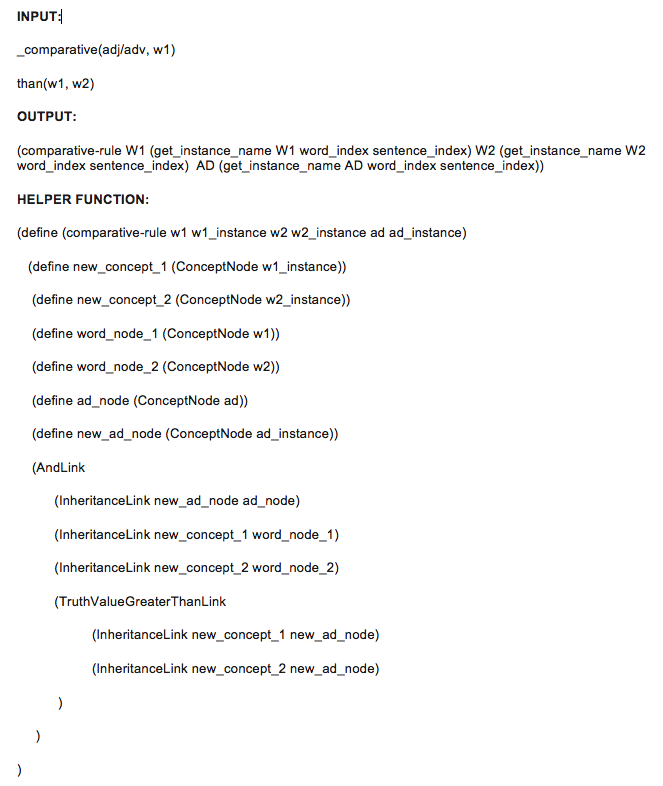
\includegraphics[width=15cm]{figures/comparativeRule.png}
\protect\caption{\label{fig:comparativeRule}Full RelEx2Logic rule for parsing one type of comparative sentence.}
\end{centering}
\end{figure*}

使用这个规则的一个简单例子是:

{\tt\begin{small}\begin{lstlisting}
Pumpkin is cuter than the white dog.
==>
_predadj(cute, Pumpkin)
than(Pumpkin, dog)
_comparative(cute, Pumpkin)
_amod(dog, white)
==>
AndLink
   InheritanceLink dog_11 white
   InheritanceLink dog_11 dog
   TruthValueGreaterThanLink
       InheritanceLink Pumpkin cute
       InheritanceLink dog_11 cute
\end{lstlisting}\end{small}}

另一方面,为了处理诸如“Amen is more intelligent than insane”这样的句子,我们使用一个不同的规则,这个规则的简短形式如下:

{\tt\begin{small}\begin{lstlisting}
_predadj(adj1, W)
than(adj1, adj2)
_comparative(adj1, W)
==>
TruthValueGreaterThanLink
    InheritanceLink W adj1
    InheritanceLink W adj2
 \end{lstlisting}\end{small}}
 
结果输出如下:

 {\tt\begin{small}\begin{lstlisting}
_predadj(intelligent, Amen)
than(intelligent, insane)
_comparative(intelligent, Amen)
==>
TruthValueGreaterThanLink
     InheritanceLink Amen intelligent
     InheritanceLink Amen insane
 \end{lstlisting}\end{small}}

%%%%%%%%%%%%%%%%%%%%%%%%%%%
\section{在简单句子集的性能评价}{Performance Evaluation of Comprehension Pipeline on Simple Sentences}
%%%%%%%%%%%%%%%%%%%%%%%%%%%


由于本文中的自然语言理解系统最终输出的基于超图逻辑形式比较独特,无法与其他类似系统进行比较。这里我们从路透社的语料库中随机抽取了100个词数小于8的句子作为测试集(选择相对较短句子来作为测试集,我们的出发点在于着重测试该自然语言理解系统对词语或短语之间的语义关系,而非专注于处理复杂的语言现象),在上面运行了我们的自然语言处理系统,并对输出结果做了人工分析,评价结果可参见下表:


\FloatBarrier

\begin{table}
\center
\begin{tabular}{|r|r|r||c|}
\hline
 & Link Parser\\
\hline
完全正确 & 96   \\
几乎正确 & 2    \\
错误 & 2       \\

\hline
\end{tabular}
\caption{改进后的链语法分析器在该测试集上的分析结果。“几乎正确”是指分析结果中忽略了链语法词典中不存在的词,但对剩下部分解析正确。}
\label{table:settings}
\end{table}


\begin{table}
\center
\begin{tabular}{|r|r|r||c|}
\hline
 & RelEx\\
\hline
完全正确 & 80    \\
几乎正确 & 15     \\
错误 & 1     \\

\hline
\end{tabular}
\caption{在链语法分析器解析完全正确的96个句子上,RelEx的性能分析。其中“几乎正确”是指输出中忽略或错误输出了1个以内的依存关系。}
\label{table:settings}
\end{table}

\begin{table}
\center
\begin{tabular}{|r|r|r||c|}
\hline
 & RelEx2Logic\\
\hline
完全正确 & 68    \\
几乎正确 & 12     \\
错误 & 0     \\

\hline
\end{tabular}
\caption{在链语法分析器和RelEx都解析完全正确的80个句子上,RelEx2Logic的性能分析。其中“几乎正确”是指输出中忽略或错误输出了1个以内的语义关系。'}
\label{table:settings}
\end{table}

\FloatBarrier


在该测试集中,链语法解析器唯一解析完全失败的句子是:

\begin{verbatim}
But can one, really?
\end{verbatim}

\noindent 在该测试集中,很多改进后的链语法解析器没有完全解析正确的句子,主要是因为对习语的分析错误,如:

 \begin{verbatim}
It has held them at bay.
 \end{verbatim}

\noindent (这里的``at bay'并不是字面意义的“bay”').


在该测试集中,RelEx分析完全失败的也只有1句:

 \begin{verbatim}
Part of it is, of course
 \end{verbatim}
 
 \noindent 其输出如下:

 \begin{verbatim}
Error: No target! rel=_pobj and src=of
    _advmod(be, of_course)
    _subj(be, it)
    _quantity(it, part)
    _det(it, part)
    _advmod(part, of)
 \end{verbatim}'
 
\noindent  但也有一些情况,RelEx忽略了很重要的依存关系,如:

 \begin{verbatim}
The expression has become quite a cliche.
\end{verbatim}

输出中只有下列依存关系:

 \begin{verbatim}
   _obj(become, cliche)
    _subj(become, expression)
   \end{verbatim}'
     
同时还有下列属性:

 \begin{verbatim}
    pos(quite_a, det)
    idiom-FLAG(quite_a, T)
   \end{verbatim}'
     
\noindent 该例中,RelEx忽略了``quite a'' 和"cliche'之间的依存关系;

 类似,在该测试集上,RelEx2Logic也几乎都给出合理的语义关系,但有时的输出也不完整。如:

  \begin{verbatim}
 But there is also compassion. 
    \end{verbatim}'
 
 \noindent RelEx2Logic没有产生与”but“相关的语义关系,这是因为有关“but”的RelEx2Logic规则还没写入规则库
it does not produce a relation for ``but'' because at this time no ``but'' rule has been coded.   Similarly in
 
总的来说,在该简单的测试集上的结果是鼓舞人心的,它能说明,本章阐述的自然语言系统在简单句子上的表现性能是不错的,其中大部分错误也都能通过添加相关的规则来解决。当然,基于规则的系统的本质也在于能通过不断添加和修改规则来提高系统的性能,但总归是很耗时的,而且也很不灵活,因此,我们希望能使机器自动从无标注或者半标注的语料库中学习相关的语法规则来替换我们所使用的人工编写的规则库。本文第\ref{chap:learning}章也提出了一个无监督的语言学习的思路。

%%%%%%%%%%%%%%%%%%%%%%%%%%%%%%%%%%%%%%%%%%%%%%%%%%%%%%%%%%%%%%%
\section{本章小结}{Summary of Accomplishments and Future Work}
%%%%%%%%%%%%%%%%%%%%%%%%%%%%%%%%%%%%%%%%%%%%%%%%%%%%%%%%%%%%%%%

本章主要介绍我们的自然语言理解系统中的各个模块的工作原理和实现方法,并深入讨论了该系统如何将英文句子转换成超图表示的逻辑形式,以达到能使自然语言参与到逻辑推理的过程中。该自然语言理解系统已经被应用在游戏角色控制和人形机器人等领域。

该自然语言理解系统使用了一些现有的开源语法分析器,本章也讨论对这些开源工具做出的各种改进,还讨论了我们实现的全新的将依存关系转换成语义逻辑表示的系统RelEx2Logic,总的来说,本章的贡献有:

\begin{itemize}
\item 改进了链语法分析器的词典,使其能够处理更复杂的语言现象,以及能识别句子的中心词从而改进了链语法对复句的分析能力。
\item 改进了RelEx使其能处理目前语法分析器难以处理的比较级和量词等复杂的语言现象。
\item 设计并实现了RelEx2Logic系统,使其能将RelEx输出的依存关系转换成以超图表示的逻辑形式
\item 设计并实现了RelEx2Logic中所使用的转换规则及相应的规则引擎。
\end{itemize}

总的来说,本章搭建的自然语言理解系统已经能被用在一些用户定义的实际应用中,但仍然有很多遗留问题有待解决。在接下来的工作中,我们会在我们的自然语言理解系统中引入概率逻辑推理引擎PLN,这样不仅可以通过一些基本常识推理来改进语法分析中的结果,还可用于指导对语法分析器产生的多种结果进行排序,以及用于指导各种歧义消除和指代消解等方面。除此之外,我们还致力通过无监督的机器学习方法从大型文本语料学习相关的语法规则,来替代当前系统中使用的人工编写的规则库,本文会在第\ref{chap:learning}章中对此做更深入的讨论。最后,本章还在一个小的测试集上对我们的自然语言理解系统进行了测试并做了相应的评价分析。



